\section{نتایج}

برای ارزیابی جامع روش‌های درون‌یابی، آزمایش‌ها با دو بازه آموزشی متفاوت [1950, 2020] و [1960, 2010] انجام شد. بازه اول کل دوره مورد نظر را پوشش می‌دهد و بازه دوم بر بخش مرکزی داده‌ها تمرکز دارد. این رویکرد امکان بررسی عملکرد روش‌ها در درون‌یابی (درون بازه آموزش) و برون‌یابی (خارج از بازه آموزش) را فراهم می‌کند و به درک بهتر پایداری و حساسیت هر روش نسبت به مرزهای داده کمک می‌کند.

شکل‌های \ref{fig:forward}-\ref{fig:regression} نتایج درون‌یابی با هر روش را در بازه کامل [1950, 2020] نشان می‌دهند. شکل‌های \ref{fig:forward2}-\ref{fig:regression2} نتایج زمانی که مدل‌ها فقط روی بازه [1960, 2010] آموزش دیده‌اند (و برای سال‌های خارج از این بازه برون‌یابی انجام می‌دهند) را نمایش می‌دهند.

\begin{figure}[htbp]
    \centering
    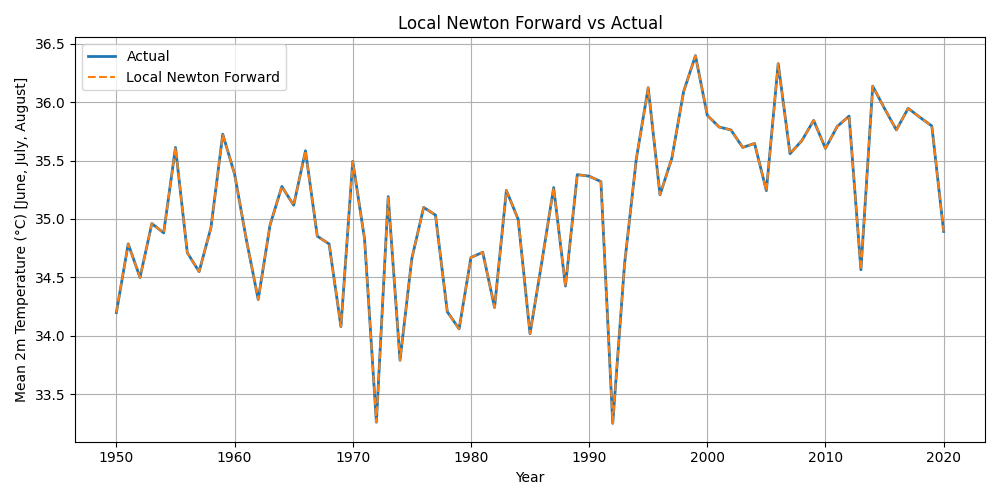
\includegraphics[width=0.8\textwidth]{../figs/Local_Newton_Forward_vs_actual[1950, 2020, 1].png}
    \caption{درون‌یابی نیوتن پیشرو محلی در مقایسه با داده واقعی (1950 تا 2020)، آموزش‌دیده روی بازه [1950, 2020]}
    \label{fig:forward}
\end{figure}

\begin{figure}[htbp]
    \centering
    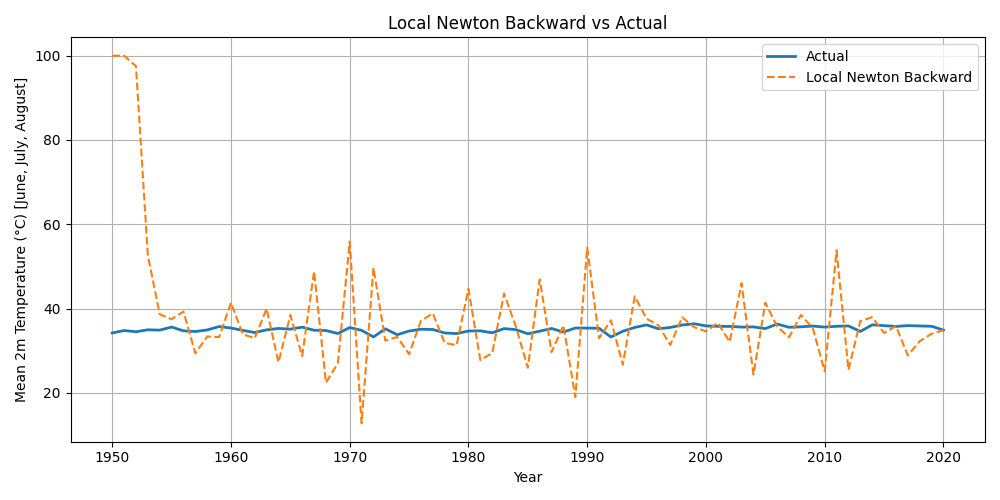
\includegraphics[width=0.8\textwidth]{../figs/Local_Newton_Backward_vs_actual[1950, 2020, 1].png}
    \caption{درون‌یابی نیوتن پسرو محلی در مقایسه با داده واقعی (1950 تا 2020)، آموزش‌دیده روی بازه [1950, 2020]}
    \label{fig:backward}
\end{figure}

\begin{figure}[htbp]
    \centering
    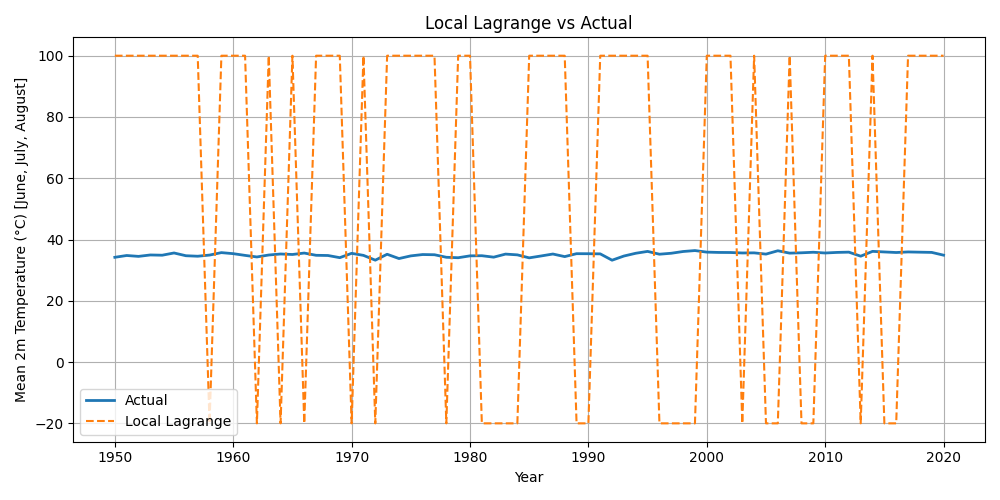
\includegraphics[width=0.8\textwidth]{../figs/Local_Lagrange_vs_actual[1950, 2020, 1].png}
    \caption{درون‌یابی لاگرانژ محلی در مقایسه با داده واقعی (1950 تا 2020)، آموزش‌دیده روی بازه [1950, 2020]}
    \label{fig:lagrange}
\end{figure}

\begin{figure}[htbp]
    \centering
    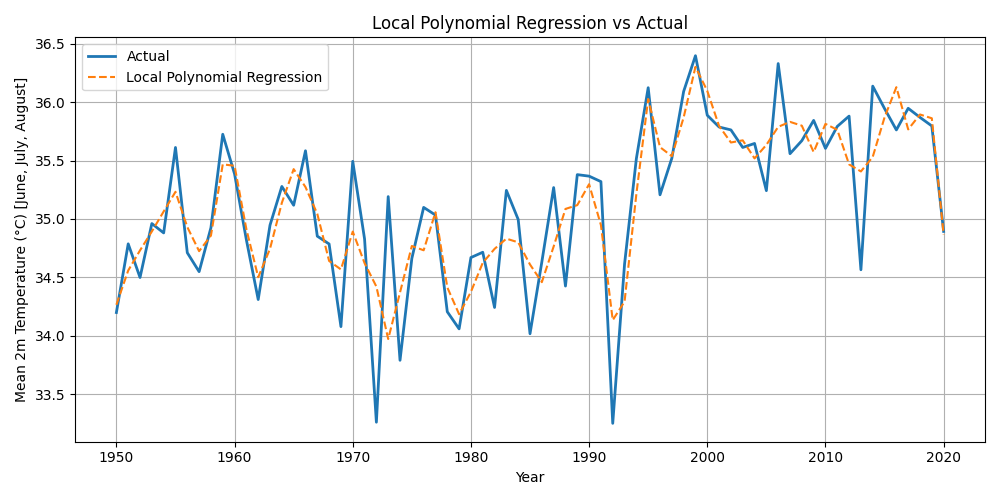
\includegraphics[width=0.8\textwidth]{../figs/Local_Polynomial_Regression_vs_actual[1950, 2020, 1].png}
    \caption{رگرسیون چندجمله‌ای محلی در مقایسه با داده واقعی (1950 تا 2020)، آموزش‌دیده روی بازه [1950, 2020]}
    \label{fig:regression}
\end{figure}

\begin{figure}[htbp]
    \centering
    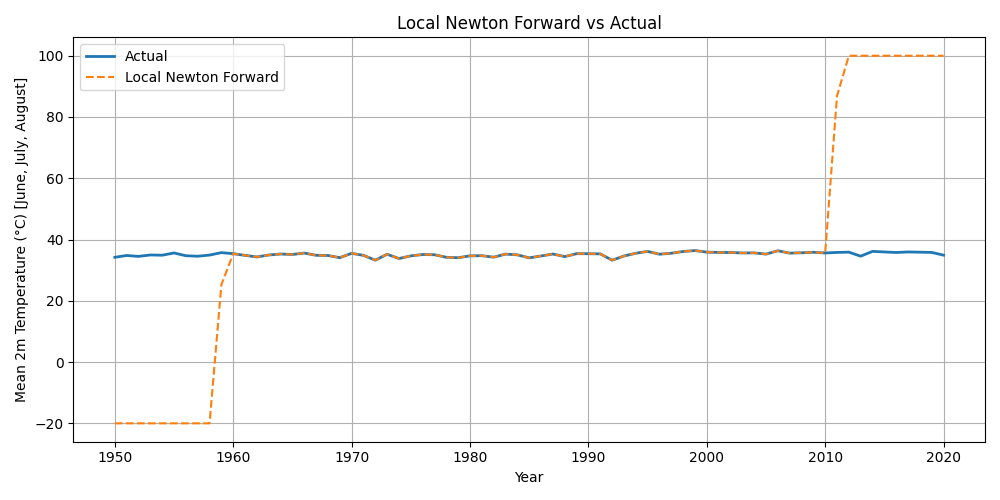
\includegraphics[width=0.8\textwidth]{../figs/Local_Newton_Forward_vs_actual[1960, 2010, 1].png}
    \caption{درون‌یابی نیوتن پیشرو محلی در مقایسه با داده واقعی (1950 تا 2020)، آموزش‌دیده روی بازه [1960, 2010]}
    \label{fig:forward2}
\end{figure}

\begin{figure}[htbp]
    \centering
    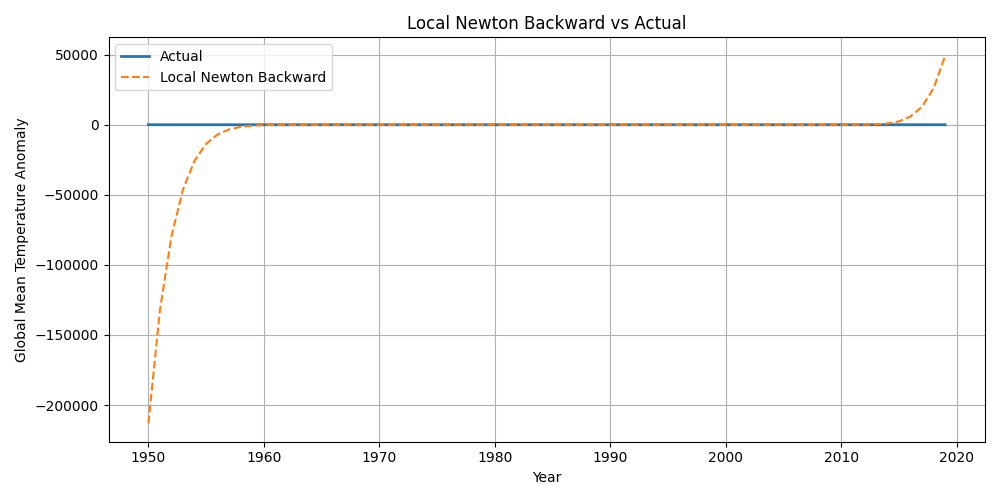
\includegraphics[width=0.8\textwidth]{../figs/Local_Newton_Backward_vs_actual[1960, 2010, 1].png}
    \caption{درون‌یابی نیوتن پسرو محلی در مقایسه با داده واقعی (1950 تا 2020)، آموزش‌دیده روی بازه [1960, 2010]}
    \label{fig:backward2}
\end{figure}

\begin{figure}[htbp]
    \centering
    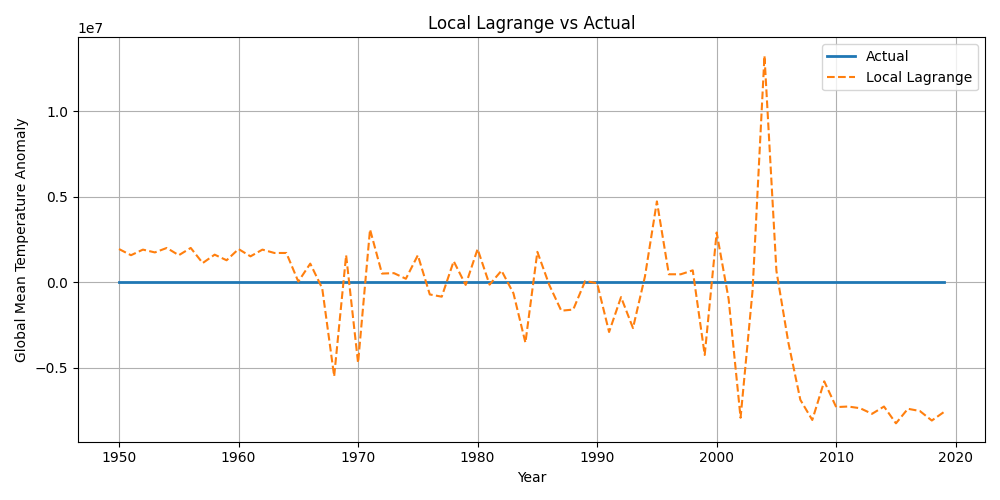
\includegraphics[width=0.8\textwidth]{../figs/Local_Lagrange_vs_actual[1960, 2010, 1].png}
    \caption{درون‌یابی لاگرانژ محلی در مقایسه با داده واقعی (1950 تا 2020)، آموزش‌دیده روی بازه [1960, 2010]}
    \label{fig:lagrange2}
\end{figure}

\begin{figure}[htbp]
    \centering
    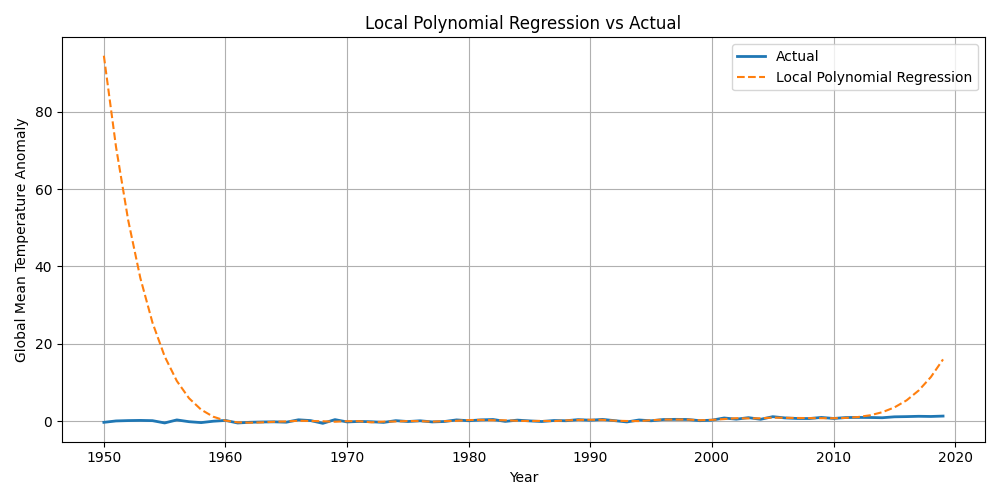
\includegraphics[width=0.8\textwidth]{../figs/Local_Polynomial_Regression_vs_actual[1960, 2010, 1].png}
    \caption{رگرسیون چندجمله‌ای محلی در مقایسه با داده واقعی (1950 تا 2020)، آموزش‌دیده روی بازه [1960, 2010]}
    \label{fig:regression2}
\end{figure}

\begin{table}[htbp]
    \centering
    \begin{tabular}{lcc}
        \hline
        روش & RMSE (1950--2020) & RMSE (1960--2010) \\
        \hline
        نیوتن پیشرو محلی & 0.00000 & 16210.40502 \\
        نیوتن پسرو محلی & 64.87515 & 32854.40094 \\
        لاگرانژ محلی & 3949913.66296 & 4109505.16614 \\
        رگرسیون چندجمله‌ای محلی & 0.18621 & 16.67956 \\
        \hline
    \end{tabular}
    \caption{ریشه میانگین مربعات خطا (RMSE) برای هر روش و هر بازه آموزشی.}
    \label{tab:rmse}
\end{table}
